\documentclass[12pt]{article}

%% preamble: Keep it clean; only include those you need

% if the below packages cannot be installed automatically, you can 
% download the required .sty files from CTAN and place them in the
% same location as the .tex file (or upload to overleaf in same
% location (folder) in overleaf

\usepackage{amsmath}
\usepackage[margin = 1in]{geometry}
\usepackage{graphicx}
\usepackage{booktabs}
\usepackage{natbib}
\usepackage{float}

\usepackage{lineno}  % use these two lines to include line numbers
\linenumbers

\usepackage{setspace} % for doublespacing
\doublespacing


% highlighting hyper links
\usepackage[colorlinks=true, citecolor=blue]{hyperref}


\usepackage{color}
\newcommand{\blue}{\color{blue}} 
% when you make your edits in response to review/instructor comments, 
% you can indicate changes in color

%% meta data

\title{A Statistical Analysis of Real Estate Trends in Connecticut}
\author{Nathan Nhan\\
  Department of Statistics\\
  University of Connecticut
}

\begin{document}
\maketitle

\begin{abstract}
This paper presents an applied statistical analysis of real estate sales trends in Connecticut over the past two decades. The objective of this analysis is to identify any significant trends that may have led to spikes or declines in the real estate market during this time period. To achieve this, data science techniques in python such as the Kruskal-Wallis test were used to determine if the difference in medians of the sales ratio variable and the medians of the amount of sales per year were statistically significant. The applications of this research can provide valuable insights into the factors affecting the real estate market in Connecticut. These insights can be used by real estate professionals, policymakers, and investors in the CT area.

\noindent\textbf{Keywords}: Dunn's Test, economy, Kruskal-Wallis test, market, real estate, Wilks-Shapiro test
\end{abstract}



\newpage
\section{Introduction}
\label{sec:intro}

The general economy and the real estate market of the United States are forever interlinked. The economic factors such as the health of the national market (usually measured by the Gross Domestic Product Growth also known as GDP Growth), employment rates, and consumer confidence, directly affects the demand and supply of real estate. This in turn affects every individual consumer. To explain this bluntly: when the economy is doing well, more people have more disposable income, which leads to increased demand for homes, commercial buildings, and other products in the real estate market. Conversely, when there is an economic downturn, the demand for products such as real estate decreases, resulting in lower prices and slower growth in many industries. In addition to this connection, real estate sales and other connecting industries, such as construction work and finance, provide employment and generate revenue for both the state and country. In fact, according to \citep{Quigley} there have been many studies throughout the history of the United States that suggest that "construction and price development were synchronized with long swings in aggregate economic activity." These long swings in the economy are defined as periods of economic growth followed by economic recession that can last from either several years to even decades. Studying and analyzing these long swings in aggregate economic activity is important as it can provide insights into the underlying drivers of economic growth and stability. 

Specific details from these studies such as those mentioned by \citep{Quigley} include detailed analyses of economic fundamentals in the context of aggregate United States national housing price trends, which are then applied to specific regions of the country. However, as stated by \citep{Quigley}, very few of these models have been generalized and applied to explain price movements across general local areas. To fill this gap of knowledge, this study uses a dataset that reflects a general local area, in this case the 3rd smallest state in the country, Connecticut. The hope in this analysis is to find trends that reflect the same trends found in these national studies.

Now that we've established that the economy and real estate markets are interlinked with one another, we can also then connect the real estate market to population growth. Zero population growth is defined as a "condition in a population where the number of births matches the number of deaths and therefore there is no net increase" by \citep{Robbins}. This phenomenon is cited as the ideal condition for the economy as the demand for houses remain constant and not ever increasing. Too much of a demand for homes causes the supply and demand balance of the housing market to become lopsided. While zero population growth is the ideal, the United States instead the phenomenon known as a positive population growth. This is where the amount of births of a population outweigh the amount of deaths. Recent predictions, using data from prior censuses in the U.S., have the population of the United States growing from around 319 million in 2014 to 417 million by 2060. This growth is estimated to require over 38 million additional housing units, according to \citep{saiz2017real}, to properly house all these new individuals. To put things into perspective, the Census estimates that 2010-2016 show an average of only 665,000 new housing units being added a year. According to \citep{Williams}, many commentators believe that this will create a housing crisis for the United States.

These concerning statistics bring more evidence to the importance for lawmakers, politicians, and real estate professionals to able to identify the clear issues with the vulnerability of the real estate market and be able to properly fight back against these looming concerns. In addition, these statistics can also assist both prospecting families and real estate moguls so that they can identify when the real estate market is at its healthiest in order to buy the best properties at the best prices.

In order to assist these demographics, we can analyze real estate trends to help predict the state of the real estate market. For instance, the COVID-19 pandemic brought sweeping changes to the economy that can still be felt to this today. The goal of this paper is to analyze what factors specifically have led to these changes in real estate market so that readers of this study can better understand and prepare for any wide-sweeping changes in the housing market. 
Such an analysis of the real estate market is not just important for the real estate market itself, but for the economy as well. This data analysis details the impact on individual and business investments during times of both economic growth and downturn, and its susceptibility to external factors. These factors can be later studied to prepare lawmakers and even individuals to prepare themselves against further recessions or future potential pandemics, so that they can stay one step ahead of the real estate market.

With all this in mind, the hypothesis of this paper is that there was a statistically significant impact on the amount of sales and profits from real estate listings during the COVID-19 pandemic. Specifically, a question that a real estate agent may ask when looking to get into the real estate market is if 2020 was significantly different than previous years in terms of both amount of listings and the sales ratio of those listings. These two variables can help indicate to that agent on whether or not it's more important to get more sales versus getting a higher profit margin for sales when starting out in real estate.

What I expect to see in this analysis is that the mean of the sales ratio in 2020 was statistically greater than that of the later years. In addition to this, I believe that the amount of sales would be statistically significant as since the economy took a hit during the pandemic, then it would stand to reason that the amount of real estate listings would increase as people would be needing more money and thus would need to downsize their living environment.

% roadmap
The rest of the paper is organized as follows. The data will be presented in 
Section~\ref{sec:data}. Section~\ref{sec:meth} describes the Methods. Section~\ref{sec:meth} describes the Results. A discussion concludes in Section~\ref{sec:disc}.


\section{Data Description}
\label{sec:data}

\begin{figure}[!t]
  \centering
  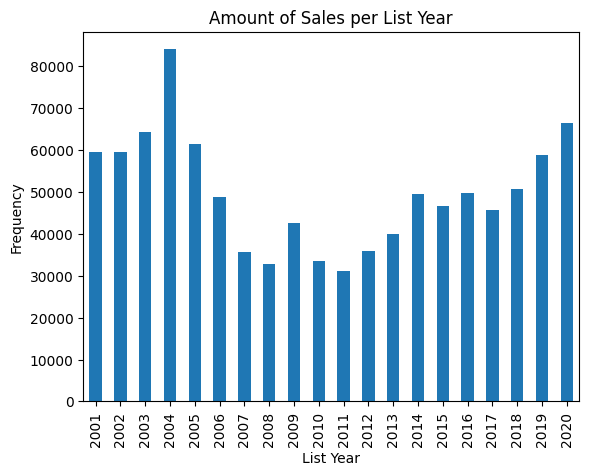
\includegraphics[width=\textwidth]{YearFreq.png}
  \caption{Bar chart graph of the frequency of real estate sales for each list year}
  \label{fig:YearFreq}
\end{figure}

\begin{figure}[!t]
  \centering
  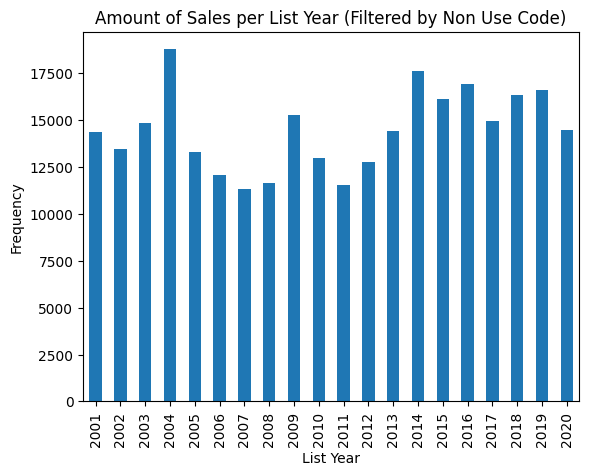
\includegraphics[width=\textwidth]{YearFreq2.png}
  \caption{Bar chart graph of the frequency of real estate sales for each list year factoring in the Non Use Code column}
  \label{fig:YearFreq2}
\end{figure}

The data is pulled from The Office of Policy and Management on the official Connecticut State website  \href{data.ct.gov/Housing-and-Development/Real-Estate-Sales-2001-2020-GL/5mzw-sjtu}{data.ct.gov} \citep{realestatedata}. This dataset contains a list of listings of corresponding real estate sales in Connecticut that occurred between the dates of October 1st and September 30th of each list year (the year the houses was listed for sale) from 2001-2020. Any real estate sales that fall below the price of \$2000 are not included. While the list year was between 2001-2020, the data for sold homes/condos is continually updated with relevant sales data up to October 2022. The decision to base the Real Estate sales solely on Connecticut real estate listing was to reflect the location and University (University of Connecticut) that this analysis was written for.

Some relevant columns in the dataset are the \textit{Sale Date}, \textit{Property Type} (either residential, an apartment, commercial, industrial, or vacant land), the \textit{Residential Type }(indicates whether property is single or multifamily residential), and finally the trio of sales columns. The sales are split into three separate columns: \textit{Assessed Value}, \textit{Sale Amount}, and \textit{Sales Ratio}. The Assessed Value is the value of the property used for local tax assessment. The Sale Amount is the amount the property was sold for. Finally the Sales Ratio is the ratio of the sale price to the assessed value. 

A particularly relevant column was the \textit{Non Use Code} which indicates whether or not the particular listing's sale price was not reliable for use in the determination of a property value. Explanations for why the Non Use Code is present is contained in the two unused columns: \textit{Assessor Remarks} and \textit{OPM remarks}.


Figure~\ref{fig:YearFreq} is a frequency table represented as a histogram that distributes the amount of separate real estate sales per year. From Figure~\ref{fig:YearFreq}, we can see that 2004 was the year that contained the most amount of listing of housings followed by 2020. The least amount of listings belongs to the year 2011. 

However, this data is not reflective in regards to the usage of the \textit{Non Use Code} column. If we factor in the use of the \textit{Non Use Code} column, our data can now be represented by Figure~\ref{fig:YearFreq2}. Here, 2004 is still the list year with the highest frequency of real estate listings. However, we can see that 2020 significantly declined in frequency compared to the frequency found in Figure~\ref{fig:YearFreq}. Instead, Figure~\ref{fig:YearFreq2} shows us that the year 2014 is the second highest frequent list year for new real estate listings. The least frequent list year in the filtered graph is 2007. 


\begin{table}[!t]
\caption{Descriptive Statistics of the Net Profit (Sale Price - Assessed Value) for each List Year}
\label{tab:dsSR} 
\centering
\begin{tabular}{r|r|r|r|r}
\toprule
List Year & Count & Mean & Std Dev & Median \\
\midrule
2001 & 14359.0 &   49416.627342 & 8.711551e+05 &  35400.0 \\
2002 & 13438.0 &  -15055.606117 & 1.616562e+06 &  41040.0 \\
2003 & 14845.0 &   29909.321320 & 1.979192e+06 &  66860.0 \\
2004 & 18757.0 &   20305.782694 & 1.899343e+06 &  76900.0 \\
2005 & 13288.0 &   47896.930990 & 1.640954e+06 & 106130.0 \\
2006 & 12092.0 &  -91472.639315 & 3.335053e+06 &  85500.0 \\
2007 & 11302.0 &  -68448.820032 & 2.844138e+06 &  41830.0 \\
2008 & 11623.0 &  -80627.173879 & 2.407182e+06 &   -300.0 \\
2009 & 15266.0 & -138780.333879 & 2.660207e+06 & -12900.0 \\
2010 & 12975.0 &  -79102.245703 & 1.146645e+06 & -18750.0 \\
2011 & 11561.0 & -244327.171698 & 3.255517e+06 & -22370.0 \\
2012 & 12735.0 & -135314.557815 & 2.724851e+06 &  -4910.0 \\
2013 & 14430.0 &  -65396.872488 & 3.238957e+06 &  -2905.0 \\
2014 & 17584.0 &  -26783.593342 & 1.996485e+06 &  -2700.0 \\
2015 & 16121.0 & -125337.990633 & 2.469163e+06 &   -400.0 \\
2016 & 16942.0 &  260925.334140 & 8.990827e+06 &   7385.0 \\
2017 & 14963.0 & -113811.553996 & 7.676327e+06 &  15450.0 \\
2018 & 16354.0 &  -40474.385703 & 2.558964e+06 &  22415.0 \\
2019 & 16596.0 &   13136.853761 & 2.956733e+06 &  39910.0 \\
2020 & 14450.0 &  528141.117436 & 4.190760e+07 &  85550.0 \\
\bottomrule
\end{tabular}
\end{table}

Next, we can determine the descriptive statistics of the Sales Ratio from Table~\ref{tab:dsSR}. This table shows us which list years produced the highest and lowest results in real estate sales based on the a newly created Net Profit metric which was calculated by performing the following equation: 

\begin{equation}
N = S - V,
\label{tab:eqProfit} 
\end{equation}
where:
\begin{itemize}
\item $S$ stands for the sale price,
\item $V$ is the assessed value,
\item $N$ stands for the Net Profit.
\end{itemize}

We see from Table~\ref{tab:dsSR} that the \textit{}{Means} with a negative sign indicate that there was an average loss of real estate value from the original assessed value. Conversely, the means that are positive indicate an average profit from the selling of the real estate listings.

Finally, there were a number of columns that went unused by this analysis. These columns include the name of the \textit{Town}, \textit{Address}, the \textit{Location's Coordinates}, and \textit{Serial Number} of the sale. These columns go unused for our dataset since many of these categorical variables were irrelevant to the the hypothesises of this paper. 


\section{Methods}
\label{sec:meth}

\begin{figure}[!t]
  \centering
  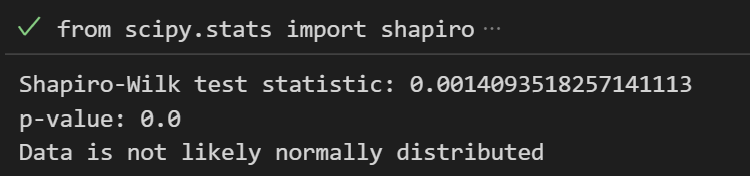
\includegraphics[width=\textwidth]{ShapiroWilk.png}
  \caption{The output after running the Shapiro-Wilk test in Python}
  \label{fig:ShapiroWilk}
\end{figure}

Firstly, we can test if the data for the Sales Ratio is normally distributed. We can prove whether or not the data is normally distributed by performing three tests. For starters we can perform the Shapiro-Wilk test. This test compares the observed data to what would be expected if the data were normally distributed. The null-hypothesis of the Shapiro-Wilk test is that the population is normally distributed. This means that if the p value is less than the chosen alpha level, in our case 0.05, then the null hypothesis is rejected and there is evidence that the data tested are not normally distributed. Conversely, if the p value is greater than 0.05, then the we can reject the null hypothesis and state that there is evidence to suggest that the data tested is normally distributed. The formula for the Shapiro-Wilk test is as follows.

Assuming we have a random sample of size $n$ from a population with an unknown distribution:

\begin{equation}
W = \frac{(\sum_{i=1}^{n}a_i x_{(i)})^2}{\sum_{i=1}^{n}(x_{i}-\overline{X})^2}.
\label{eq:Shapiro} 
\end{equation}
where:
\begin{itemize}
\item $W$ is the test statistic,
\item $X_{(i)}$ is the $i$-th order statistic of the sample,
\item $\overline{X}$ is the sample mean,
\item $a_i$ is a constant calculated in the Equation~\ref{eq:AConstant}.
\end{itemize}

Under the null hypothesis of normality, the test statistic $W$ follows a beta distribution with parameters $\alpha = \frac{n-1}{2}$ and $\beta = \frac{1}{2}$.

Since $a_i$ is a constant, it is calculated with the follow equation:
\begin{equation}
a_i = \frac{m_i}{\sqrt{\sum_{j=1}^n m_j^2}}.
\label{tab:eqAConstant} 
\end{equation}
where:
\begin{itemize}
\item $a_i$ is a constant,
\item $m_i$ is the $i$-th moment about the sample mean.
\end{itemize}


We can perform this test in python with the pandas module in tandem with the the scipy.stats shapiro function. If we set our alpha value to be 0.05, we obtain a Shapiro-Wilk test statistic of about 0.0014 and a p-value of 0.0 as seen in Figure~\ref{fig:ShapiroWilk}. Since the p-value was found to be less than our alpha value, we can conclude that our data was not approximately normal. However, this test can be rather sensitive so there are other ways to check if the data is normally distributed. Secondly, we can perform another using quantile-quantile plots and the ggplot2 module. As seen in Figure~\ref{fig:qqplot}, the graph does not depict a straight line and therefore we can can conclude that our data is not normally distributed.



\begin{figure}[!t]
  \centering
  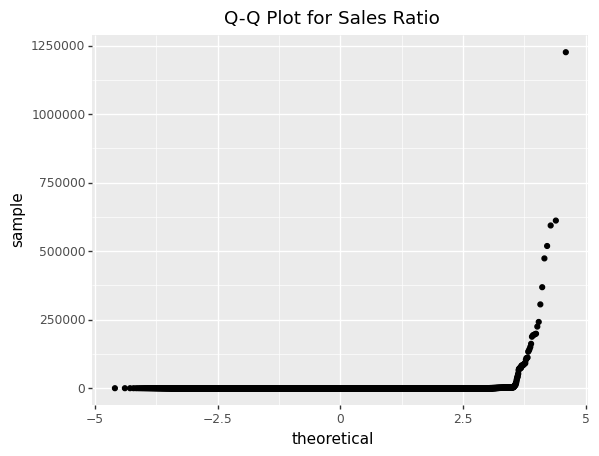
\includegraphics[width=\textwidth]{q-q plot.png}
  \caption{Q-Q Plot for the Sales Ratio used to test for Normality}
  \label{fig:qqplot}
\end{figure}

However, we can also test if the total amount of sales correlates with the list year and determine if this set of data is normally distributed. We can use the graph of the frequency to test for normality. If the graph has a bell-shaped distribution, we can then conclude that our data is normally distributed. We can again look at Figure~\ref{fig:YearFreq2} to see if the data is normally distributed. We use the filtered by non-use code graph in order to get the most accurate set of data. We see from this graph there is not much shape in it and therefore say that the our data is not normally distributed.


\begin{figure}[!t]
  \centering
  
\includegraphics[width=\textwidth]{skew.png}
  \caption{The output after performing the Skew and Kurtosis functions for the frequency graph showing in Figure 1 in scipy.stats in python.}
  \label{fig:SkewKurtosis}
\end{figure}

We can additionally use the skew and kurtosis functions from the scipy.stats module in order to see if there are any outliers prevent the graph from being normally distributed. By using the functions above, shown in Figure~\ref{fig:SkewKurtosis}, we can see that it results in the skewness equal to 0.21 and kurtosis of the graph equal to -0.85. Since the skew is significantly different from zero we can say our graph is not symmetric and the kurtosis is nowhere close to 3 indicating that our data is once again not normally distributed. 

We must instead use a test that does not rely on the data being normally distributed. With that in mind we can use a non-parametric test to determine if the COVID-19 pandemic had a significant effect on the sales ratio of sales in the real estate market. We can specifically conduct the Kruskal-Wallis test as this way we can determine if the listing years significantly impacts either the sales ratio or amount of listings in anyway. 

The Kruskal-Wallis test is a non-parametric statistical test that is used to compare the medians of two or more groups. It's used when the assumptions of normality, which we found earlier to not be the case, and homogeneity of variance are not met. The test is based on the ranks of the data rather than the actual values, and it determines whether there is a significant difference between the medians of the groups. The formula to calculate the test statistic for this test is shown below:


\begin{equation}
H = \frac{12}{N(N+1)} \sum_{i=1}^{k} \frac{T_i^2}{n_i} - 3(N+1).
\label{eq:kruskalWallis} 
\end{equation}
where:
\begin{itemize}
\item $H$ is the Kruskal-Wallis test statistic,
\item $N$ is the total sample size,
\item $k$ is the number of groups being compared,
\item $n_i$ is the sample size for group $i$,
\item $T_i$ is the sum of the ranks for group $i$.
\end{itemize}

However before we can perform this test, we must first go over the assumptions. The assumptions of the Kruskal-Wallis test are the following. Firstly, the two variables should be measured on either an ordinal, interval or ratio scale. Ordinal variables are variables that have an arbitrary ranking for each variable measured which include things like Likert scales (e.g., a 7-point scale from "strongly agree" through to "strongly disagree"). These are contrasted with interval/ratio variables which are measurable continuous variables such as speed. If we take a look at our data variables, we find that all our variables are measured on the interval/ratio scale.

Our second assumption is that we assume all the observations should be independent of each other. There should be no relationship between the members in each group or between groups. We can assume real estate listings are independent as the purchase of a listing is not typically dependent on other listings. 

Since both assumptions have been passed for our data, we are safe to use the Kruskal-Wallis test.
In order to perform this data analysis, we can use the python module scipy.stats and its corresponding Kruskal function. With this, we can easily calculate the test statistic $H$ shown earlier in Equation~\ref{eq:kruskalWallis}.

\begin{figure}[!t]
  \centering
  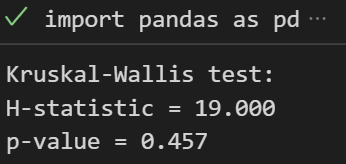
\includegraphics[width=\textwidth]{KW-SalesRatio.png}
  \caption{The output after performing the Kruskal function to test significance of the median sales ratio for each list year in scipy.stats in python.}
  \label{fig:KW-SalesRatio}
\end{figure}

With us using the Kruskal-Wallis test, we can create a hypothesis test for our data. Let us start out by comparing the medians of the sales ratio. We set our null hypothesis to that all the medians of the sales ratio were statistically similar to one another amongst all the list years. The alternative hypothesis then would be that at least one median for the sales ratio of one listing year is significantly different from the median of at least one other listing year. In addition, we set our alpha value to 0.05 

If we find that the Kruskal-Wallis test's null hypothesis test is rejected, we can perform a post-hoc test in order to directly see which list years differ from each other. Since we did the Kruskal-Wallis test, we in turn perform the non-parametric Dunn's test. The Dunn's test is as follows:


\begin{equation}
z=\frac{|\bar{r}_i-\bar{r}_j|}{\sqrt{\frac{k(k+1)}{6N}}}\sqrt{\frac{N(N+1)T}{12}}.
\label{eq:dunnTest} 
\end{equation}
where:
\begin{itemize}
\item $z$ is the test statistic,
\item $\bar{r}_i$ and $\bar{r}_j$ are the mean ranks of groups $i$ and $j$,
\item $k$ is the number of groups being compared,
\item $N$ is the total sample size,
\item $T$ is the tie correction factor.
\end{itemize}


\section{Results}
\label{sec:results}

As shown in Figure~\ref{fig:KW-SalesRatio}, we see that our H-statistic is 19.000 and the p-value is 0.457. Since our P-value was found to be greater than 0.05, we do not reject the null hypothesis. This means we do not have sufficient evidence to suggest that the median sales ratio for the listing year is statistically different between the groups.

Since we know that the frequency data for the list year was not normally distributed, we once again will use the Kruskal-Wallis test to test our data. We first set our null hypothesis to state that all the medians of the frequency for each year were statistically similar to one another. The alternative hypothesis, meanwhile, stated that at least one median would be significantly different from the median of at least one other listing year. Once again we set our alpha value to 0.05

\begin{figure}[!t]
  \centering
  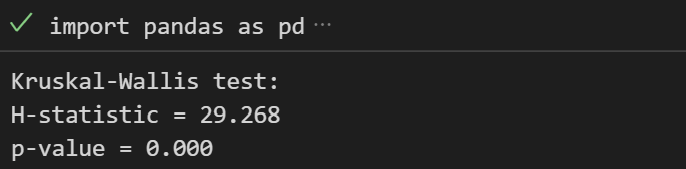
\includegraphics[width=\textwidth]{KW-Amount.png}
  \caption{The output after performing the Kruskal function to test significance of the median amount of listings for each list year in python.}
  \label{fig:KW-Amount}
\end{figure}

When we perform this test on these two variables, as seen in as seen in Figure~\ref{fig:KW-Amount}, we find that the H-statistic becomes 29.268 and the p-value to be 0.000. Since our alpha value was set to 0.05 we find that our p-value is less than our alpha. This means we can reject the null hypothesis and conclude that there is a significant difference in the median amount of sales of listings per listing year. 

Since we reject the hypothesis for the test of significant difference in the median amount of sales of listings per listing year, we can now perform the post-hoc Dunn's test for this set of data. By implementing the data into the python function posthoc\_dunn found in the python module scikit\_posthocs, we can visualize the results in Figure~\ref{fig:dunnheatmap} as a heatmap.

\begin{figure}[!t]
  \centering
  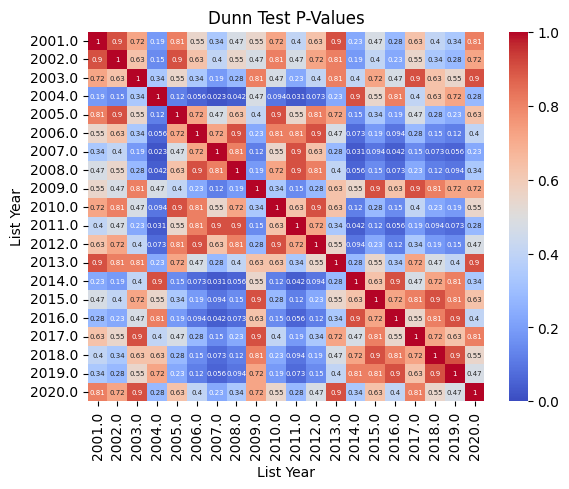
\includegraphics[width=\textwidth]{dunnheatmap.png}
  \caption{Heatmap of the results of the Dunn's test analysis}
  \label{fig:dunnheatmap}
\end{figure}

\begin{figure}[!t]
  \centering
  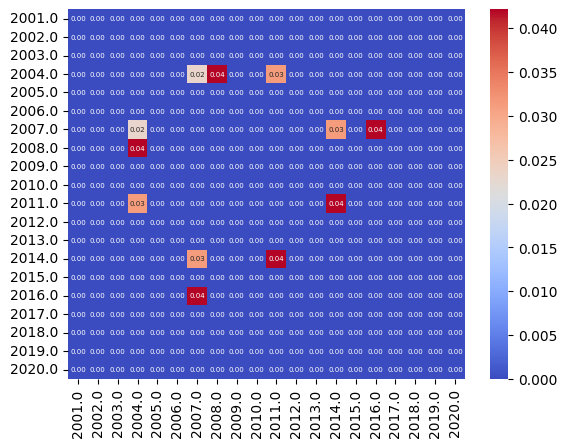
\includegraphics[width=\textwidth]{dunnheatmapmodif.png}
  \caption{Modified heatmap of the results of the Dunn's test analysis}
  \label{fig:dunnheatmapmodif}
\end{figure}

\section{Discussion}
\label{sec:disc}

The aim in this analysis was to determine whether or not the COVID-19 pandemic has any significant effect on the number of homes sold or the sales ratio of homes in the real estate market. Specifically, we wanted to determine if there was a statistical difference between the amount of sales per list year or the median sales ratio. Although the findings in the results section was inconclusive regarding whether the median sales ratios were statistically significant from one another, we did find that there was a statistically significant difference in the median amount of sales per year. This meant that we could go back to our frequency table in Figure~\ref{fig:YearFreq} and check if 2020 was a standout year.

Our analysis of the frequency table for amount of houses sold revealed that 2020 was a year with a large amount of sales. However, it was surpassed by 2004, which eclipsed 2020 with over 10,000 sales. In addition to the frequency table, we also checked the results of the post-hoc analysis to see if any of the list years had a particularly significant differences between another list year. The results of the post-hoc Dunn's test are shown in Figure~\ref{fig:dunnheatmap} and Figure~\ref{fig:dunnheatmapmodif}.In Figure~\ref{fig:dunnheatmapmodif} we set all the p-values that were greater than our significance level to zero so that we could easily tell which p-values were less than 0.05. The results showed that 2020 has no statistical differences in median between any other year and thus we cannot conclude that 2020 was a standout year. However upon further analysis, 2004, which we found surpass 2020 in our prior frequency table analysis does have statistically significant differences between other years. In particular: 2007, 2008, and 2011, we're shown to have a significant difference in median with 2004. Thus we can conclude that 2004, not 2020, is a statistically significant year the amount of real estate sales.

The fact that neither dataset was normally distributed indicates two things. Firstly, the prices of houses across the state vary wildly, which resulted in the amount of sales per list year distribution not having a bell-shaped curve. In fact, as seen in Figure~\ref{fig:YearFreq}, the frequency graph indicates a reverse bell curve. This tells us that the years during the early part of the millennia had more sales than the middle part of the 21st century so far. It then starts to climb back up after approximately the year 2011.

However, some limitations of this study include the fact that the data was not normally distributed and was obtained by listing every single significant complete sale from the real estate market. This may have occurred because there was no random sampling that happened during data collection. Additionally, the dataset only encompassed the state of Connecticut, which is not indicative of the entire country, and many of the real estate options found in this state may be dramatically different in another. Conversely, if the dataset did encompass multiple states or perhaps even the entire country, it would not be indicative of an individual state and might not be as helpful for a single legislator in CT to rely upon.

Furthermore, the dataset only comprised list years up to 2020 and did not span the later years of the pandemic such as 2021 and 2022. In a future study, it would be interesting to look at what trends we were able to see after the initial shock of the COVID-19 pandemic hit and see what variables significantly changed or mellowed out in 2021 and 2022.

This information is worth pursuing in the future as it shows us the correlations between our datasets and demonstrates to us that while 2020 was not found to be a statistically significant year, other years such as 2004, were statistically significant. The results indicate that 2004 had a more significant economic difference in the real estate market than the formally perceived 2020 which goes against the former hypothesis of this paper. This analysis can be used in future analysis as evidence that 2020 perhaps was not a significant downturn for real estate as previously thought by analysis. It is important information for legislators, lawmakers, and economists who are looking to fix or modify the nation's economic troubles to see that 2020 may not have impacted the real estate market as formally perceived. 

%\section*{Acknowledgements} %optional

\newpage

\bibliography{refs.bib}
\bibliographystyle{plainnat}


%\section*{Appendix} %optional

\end{document}